% generated by scripts/pkl_to_latex.py
% source PKL : vscan_v1_L6_Ne6_U10_t1_mode-uniform_nmin2_solver-gcg_full_restarts10_iter300_kmax5_tol1em09_V0to12_N25-ebabade1a2a1.pkl
% scan type  : vscan
% state      : gs
% quantity   : vn-entropy
% requires   : \usepackage{pgfplots} \pgfplotsset{compat=1.18}
% colours match the matplotlib PDF (tab10 cycle)
\definecolor{gmeC0}{HTML}{1F77B4}
\definecolor{gmeC1}{HTML}{FF7F0E}
\definecolor{gmeC2}{HTML}{2CA02C}
\definecolor{gmeC3}{HTML}{D62728}
\definecolor{gmeC4}{HTML}{9467BD}
\definecolor{gmeC5}{HTML}{8C564B}
\definecolor{gmeC6}{HTML}{E377C2}
\definecolor{gmeC7}{HTML}{17BECF}

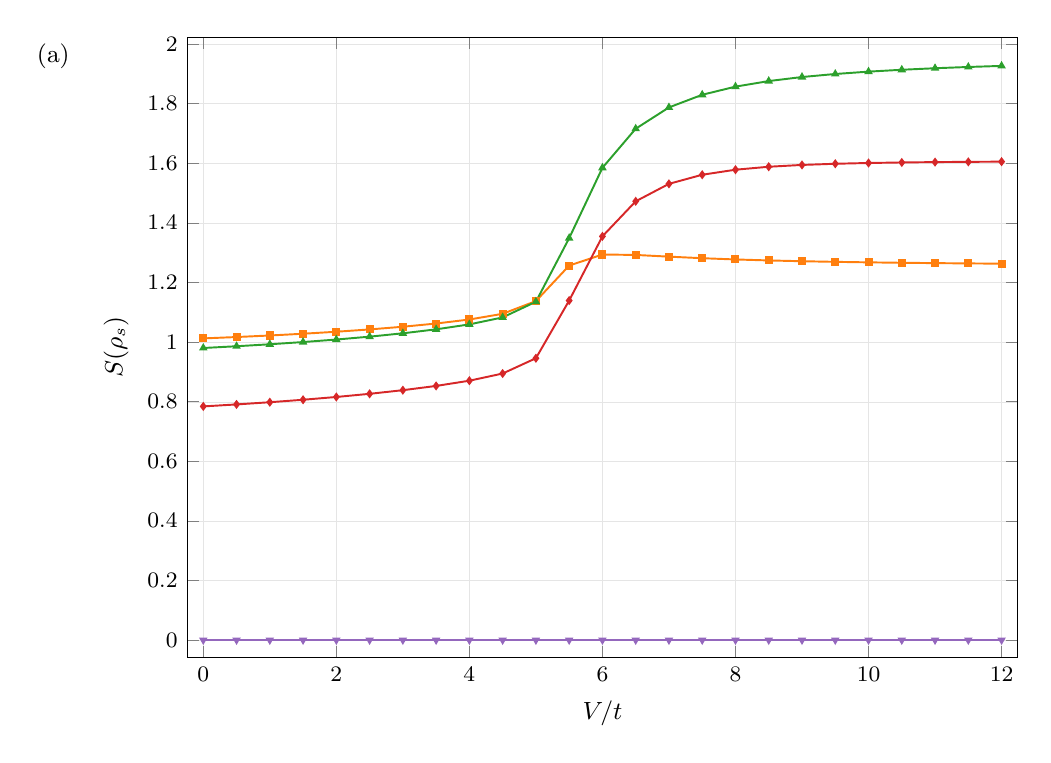
\begin{tikzpicture}
  \begin{axis}[
    width=\columnwidth,
    height=0.78\columnwidth,
    xlabel={$V/t$},
    ylabel={$S(\rho_s)$},
    grid=both,
    grid style={line width=.1pt, draw=gray!20},
    tick label style={font=\footnotesize\rmfamily, /pgf/number format/fixed},
    label style={font=\small\rmfamily},
    scaled ticks=false,
    legend style={font=\scriptsize\rmfamily, draw=gray!40, at={(0.5,1.03)}, anchor=south, /tikz/every even column/.append style={column sep=6pt}},
    legend cell align={left},
    legend columns=2,
    ymin=-0.058,
    ymax=2.023,
    xmin=-0.24,
    xmax=12.24,
    after end axis/.append code={\node[anchor=east, font=\small\rmfamily] at (axis description cs:-0.13,0.970) {(a)};},
  ]
    \addplot[color=gmeC1, mark=square*, mark size=1.1pt, line width=0.7pt] coordinates {
        (0,1.012215) (0.5,1.016807) (1,1.021989) (1.5,1.027868)
        (2,1.034581) (2.5,1.042318) (3,1.051354) (3.5,1.062147)
        (4,1.075644) (4.5,1.094741) (5,1.137418) (5.5,1.25654)
        (6,1.293729) (6.5,1.292262) (7,1.286527) (7.5,1.281305)
        (8,1.277107) (8.5,1.273796) (9,1.271172) (9.5,1.26907)
        (10,1.267364) (10.5,1.265962) (11,1.264797) (11.5,1.263819)
        (12,1.262989)
    };
    \addplot[color=gmeC2, mark=triangle*, mark size=1.1pt, line width=0.7pt] coordinates {
        (0,0.980018) (0.5,0.985906) (1,0.99251) (1.5,0.999957)
        (2,1.008409) (2.5,1.018087) (3,1.029318) (3.5,1.042653)
        (4,1.059241) (4.5,1.082634) (5,1.135314) (5.5,1.348615)
        (6,1.584663) (6.5,1.715765) (7,1.78727) (7.5,1.829693)
        (8,1.856988) (8.5,1.875731) (9,1.889271) (9.5,1.89945)
        (10,1.907351) (10.5,1.913642) (11,1.918761) (11.5,1.923)
        (12,1.926563)
    };
    \addplot[color=gmeC3, mark=diamond*, mark size=1.1pt, line width=0.7pt] coordinates {
        (0,0.784018) (0.5,0.790664) (1,0.798066) (1.5,0.806348)
        (2,0.815673) (2.5,0.826261) (3,0.838433) (3.5,0.852725)
        (4,0.870246) (4.5,0.894356) (5,0.945638) (5.5,1.139219)
        (6,1.354688) (6.5,1.472182) (7,1.530812) (7.5,1.561342)
        (8,1.578259) (8.5,1.588186) (9,1.594299) (9.5,1.598214)
        (10,1.600804) (10.5,1.602565) (11,1.603788) (11.5,1.604655)
        (12,1.605278)
    };
    \addplot[color=gmeC4, mark=triangle*, mark size=1.1pt, mark options={rotate=180}, line width=0.7pt] coordinates {
        (0,0) (0.5,0) (1,0) (1.5,0)
        (2,0) (2.5,0) (3,0) (3.5,0)
        (4,0) (4.5,0) (5,0) (5.5,0)
        (6,0) (6.5,0) (7,0) (7.5,0)
        (8,0) (8.5,0) (9,0) (9.5,0)
        (10,0) (10.5,0) (11,0) (11.5,0)
        (12,0)
    };
  \end{axis}
\end{tikzpicture}
